%%%%%%%%%%%%%%%%%%%%%%%%%%%%%%%%%%%%%%%%%%%%%%%%%%%%%%%%%%%%%%%%%%%%%%%%%%%%%%%%
%%%%%%%%%%%%%%%%%%%%%%%%%%%%%%%%%%%%%%%%%%%%%%%%%%%%%%%%%%%%%%%%%%%%%%%%%%%%%%%%
%%                          AUTHOR: BIBEKANANDA DATTA                         %%
%%                      PHD STUDENT, MECHANICAL ENGINEERING                   %%
%%                           JOHNS HOPKINS UNIVERSITY                         %%
%%%%%%%%%%%%%%%%%%%%%%%%%%%%%%%%%%%%%%%%%%%%%%%%%%%%%%%%%%%%%%%%%%%%%%%%%%%%%%%%
%%%%%%%%%%%%%%%%%%%%%%%%%%%%%%%%%%%%%%%%%%%%%%%%%%%%%%%%%%%%%%%%%%%%%%%%%%%%%%%%
\documentclass[12pt]{article}
\usepackage{blindtext}


\usepackage[utf8]{inputenc}	    %input
\usepackage[pagewise,mathlines]{lineno}


% math packages
\usepackage{amsfonts,amssymb,amsmath,dsfont,mathtools}
\allowdisplaybreaks[1]


\usepackage[ruled]{algorithm2e} % algorithm package
\usepackage[title,titletoc]{appendix}
\usepackage{autobreak}
\usepackage[english]{babel}		% for other languages
% bibliographic package


\usepackage[backend=biber, style=apa, doi=true]{biblatex}
\DeclareFieldFormat{titlecase}{#1}
\AtBeginBibliography{\urlstyle{rm}}


\usepackage[font=small,labelfont=bf,labelsep=period]{caption}
\captionsetup{belowskip=0pt}


\usepackage{color}
\usepackage{csquotes}           % for quote envionrment
\usepackage{enumitem}			% list environment
\usepackage{float}              % for image floating
\usepackage[T1]{fontenc}		% output
\usepackage[left=1in, right=1.0in, top=1.0in, bottom=1.0in]{geometry}		% margin manipulation


\usepackage{fancyhdr}
\usepackage[bottom]{footmisc}
\usepackage{graphicx,wrapfig}           %for image  
\usepackage[linktocpage, unicode, colorlinks=true, citecolor=blue, filecolor=blue, linkcolor=blue, urlcolor=blue]{hyperref}

% table related package
\usepackage{booktabs,longtable,makecell,multicol,multirow,tabularx,xltabular}



\usepackage{sectsty,titlesec}
\usepackage{setspace}           % overall spacing of the contents

\usepackage{soul}
\usepackage{tocbasic,parskip}
\usepackage{verbatim}	        %comment environemnt
\usepackage[dvipsnames]{xcolor}



%% font (comment one of the following)
%% font (comment one of the following)
\usepackage{lmodern}    	    %latin modern font
%\usepackage[sc]{mathpazo}



% %% table of content, list of table, list of figure header setting with tocbasic
\addtotoclist[\jobname]{toc}
\renewcommand \tableofcontents{\listoftoc[{\contentsname}]{toc}}
\renewcommand*{\listoffigures}{\listoftoc[\listfigurename]{lof}}
\renewcommand*{\listoftables}{\listoftoc[\listtablename]{lot}}
\setuptoc{lof}{totoc}
\setuptoc{lot}{totoc}


%% section, subsection, subsubsection, and paragraph
\setcounter{secnumdepth}{3}

\chaptertitlefont{\Large}
\chapternumberfont{\Large}

\titleformat{\section}
{\large\bfseries}{\thesection}{1em}{}[{\titlerule}]
\titleformat*{\subsection}{\normalsize\bfseries}
\titleformat*{\subsubsection}{\normalsize\sffamily}



%% no indent with single paragraph spacing
\baselineskip=12pt
\setlength{\parindent}{0pt}
\setlength{\parskip}{\baselineskip}
\setlength{\footnotesep}{0.75\baselineskip}
\setlength{\marginparwidth}{2.5cm} 
\setlength{\bibitemsep}{0.75\baselineskip}  %% bib item separation 
\def\arraystretch{1.25}
\singlespacing

%% may be useful for drafting
%\linenumbers


% Define math symbols
\numberwithin{equation}{section}
\newcommand{\vect}[1]{\mathbf{#1}}
\DeclareMathOperator{\R}{\mathrm{R}}
\DeclareMathOperator{\D}{\mathrm{D}}
\DeclareMathOperator{\tr}{tr}
\DeclareMathOperator{\divg}{div}
\DeclareMathOperator{\grad}{grad}
\DeclareMathOperator{\Grad}{Grad}
\DeclareMathOperator{\Divg}{Div}
\DeclareMathOperator{\curl}{curl}
\DeclareMathOperator{\Curl}{Curl}
\DeclareMathOperator{\sym}{sym}
\DeclareMathOperator{\skw}{skw}
\newcommand{\dC}{$^{\circ}$C}


%% for basic commenting purposes (you can add more)
\newcommand{\redtext}{\textcolor{red}}
\newcommand{\ADDCITATION}{\redtext{(ADD CITATION)}}
\newcommand{\ADDFIGURE}{\redtext{(ADD FIGURE)}}
\newcommand{\ADDTABLE}{\redtext{(ADD TABLE)}}


%% to add quote
\newcommand{\say}[2]{\hfill\small\enquote{\textit{#1}}{ - \small\textsc{#2}.}}


%% uncomment the and add the .bib file (biblatex)
% I use Zotero to generate biblatex file and include it in the same directory
%\addbibresource{phd_proposal.bib}


\begin{document}

%% BEGIN TITLE PAGE
\vspace*{0.025in}
\thispagestyle{empty}

\begin{center}
    Doctoral dissertation proposal submitted to the \\
    Department of Mechanical Engineering of The Johns Hopkins University \\
    
    \vspace{0.75in}

    \MakeUppercase{\textbf{LOREM IPSUM DOLOR SIT AMET\\CONSECTETUER ADIPISCING ELIT}}       %% tentative thesis title
    
    \vspace{0.25in}
    
    Author name   % AUTHOR (student) NAME
\end{center}

\vspace{0.75in}

% If you have more people on your committee then squeeze out some spaces or use the minipage feature
\begin{singlespace}

    \textbf{Primary advisor:}
    
    Dr. Chuck Darwin \\
    Professor \\
    Department of Biology \\
    Johns Hopkins University, Baltimore, MD \\

    \textbf{Disseration proposal committee members:} 
    
    Dr. Albrecht Einstein \\
    Professor\\
    Department of Biology \\
    Johns Hopkins University, Baltimore, MD
    
    Dr. Stewart Hawking \\
    Professor\\
    Department of Biology \\
    Johns Hopkins University, Baltimore, MD 
    
\end{singlespace}


\vspace{1in}
\begin{center}
    Baltimore, Maryland \\  % Location
    Month YEAR              % Like May 2023
\end{center}

%% END OF TITLE PAGE


%% BEGIN ABSTRACT
\newpage
\pagenumbering{roman}
\setcounter{page}{2}
\addcontentsline{toc}{section}{Abstract}
\section*{Abstract}
\blindtext


%% END ABSTRACT



%% TABLE OF CONTENT, TABLE, FIGURE
\newpage
\onehalfspacing
\renewcommand{\contentsname}{Table of Contents}
\tableofcontents


\newpage
\listoftables


\newpage
\listoffigures


%% END FRONT MATTER




%% BEGIN MAIN TEXT
\newpage
\singlespacing
\pagenumbering{arabic}



\section{Background and significance}    %% 2 page limit

\blindtext

\begin{figure}[ht]
\begin{center}
    \includegraphics[width=\textwidth, trim={6cm 5cm 6cm 5cm},clip,page=2] {proposal_figures.pdf}
    \caption{Here are some photos of ducks to make you feel happy.}
    \label{fig:ducks}
\end{center}
\end{figure}





\section{Research objectives}       %% 1 page limit

\blindtext


\phantomsection
\subsection*{Objective 1: Some major objective here}
\addcontentsline{toc}{subsection}{Objective 1: Some major objective here}

\blindtext




\section{Proposed methodology and results} %% 4 page limit

\subsection{Task 1: Major project task heading here related to objective 1}

\blindtext

\begin{figure}[ht]
\begin{center}
    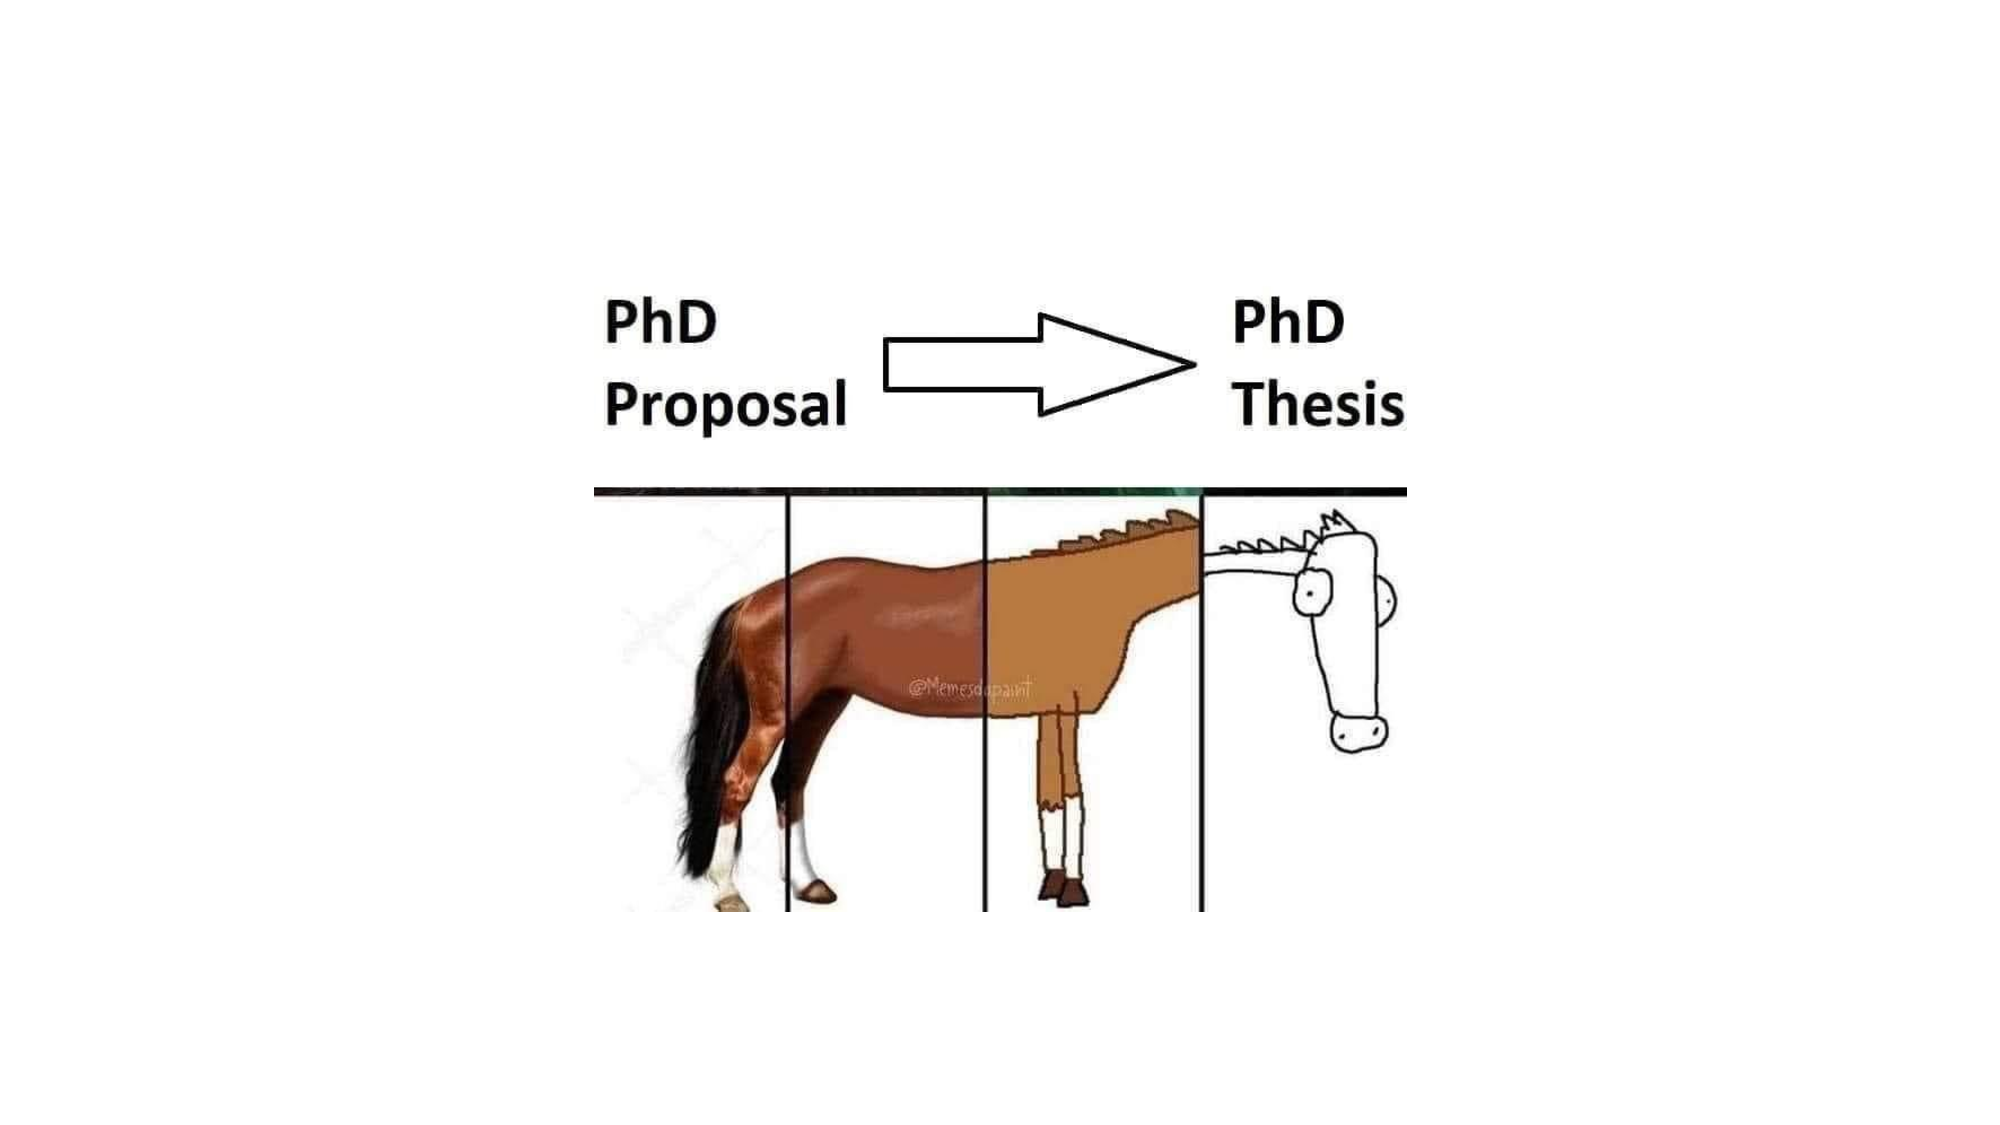
\includegraphics[width=12.5cm, trim={9cm 3cm 9cm 4cm},clip,page=1] {proposal_figures.pdf}
    \caption{Progression of project of a barely surviving PhD student.}
    \label{fig:proposal-plan}
\end{center}
\end{figure}




\subsubsection*{Subtask 1.1: Some sub-task here}
\addcontentsline{toc}{subsubsection}{Subtask 1.1: Some sub-task here}
\blindtext



\section{Planned publications}

\begin{enumerate} [leftmargin=0.75cm,itemsep=0pt]
    %
    \item %\fullcite{add_the_biblatex_tag}.
    \item %\fullcite{add_the_biblatex_tag}. \hfill (In preparation)
    \item %\fullcite{add_the_biblatex_tag}.
    %
\end{enumerate}



\section{Timeline}

%% may add a chart showing the progress



%% Optional acknowledgment section (uncomment if you want to use)
% \section*{Acknowledgement}
% \addcontentsline{toc}{section}{Acknowledgement}



\newpage
\section*{References}
%\printbibliography[heading=none] 
% Un-comment the above line once you have the bib file
\addcontentsline{toc}{section}{References}


\end{document}